\chapter{Commande des robots manipulateurs II: dynamique}

Ce chapitre présente des techniques de commande qui s'applique pour les systèmes robotisés qui peuvent être représentés par l'équation des manipulateurs décrite au chapitre \ref{sec:dynamic}.

%%%%%%%%%%%%%%%%%%%%%%%%%%%%%%%%%%%%%%%%%%%%%%%%%%%%%%%
\section{Introduction à la commande des manipulateurs}
%%%%%%%%%%%%%%%%%%%%%%%%%%%%%%%%%%%%%%%%%%%%%%%%%%%%%%%

\video{Introduction à la commande des robots}{https://youtu.be/eL6i319X_w4}

\video{L'espace des phases}{https://youtu.be/eL6i319X_w4}

\video{Tour d'horizon des méthodes de commande dans l'espace des phases}{https://youtu.be/eL6i319X_w4}

\colab{Testez votre loi de commande pour un manipulateur}{https://colab.research.google.com/drive/1bnJ9v5kHRFFhnNOZx-_Kcht2l5sTOHxr?usp=sharing}

\video{Grandes familles de méthodes de commande pour gérer l'incertitude}{https://youtu.be/hbZBF-OEZEw}


\newpage
%%%%%%%%%%%%%%%%%%%%%%%%%%%%%%%%%%%%%%%%%%%%%%%
\section{Commande dé-localisée}
%%%%%%%%%%%%%%%%%%%%%%%%%%%%%%%%%%%%%%%%%%%%%%%

\colab{Simulation d'un manipulateur avec des PIDs }{https://colab.research.google.com/drive/1qaCNY2ohQIbC6dV2ZW4KY6FDM9NhJzH2?usp=sharing}


\newpage
%%%%%%%%%%%%%%%%%%%%%%%%%%%%%%%%%%%%%%%%%%%%%%%%%%%%%
\section{Commande avec la méthode du couple calculé}
%%%%%%%%%%%%%%%%%%%%%%%%%%%%%%%%%%%%%%%%%%%%%%%%%%%%%

La méthode du couple calculé consiste à utiliser les équations d'un modèle dynamique d'un système robotique pour déterminer les forces à appliquer pour obtenir une accélération cible. Il est ensuite possible de calculer cette accélération cible de sorte à converger vers la position ou trajectoire désirée.

\video{Méthode du couple calculé}{https://youtu.be/QuEhwAUxx5Y}


\subsection{Commande de l'accélération des joints}

Premièrement, si un système est pleinement actionné, il est possible d'imposé d'une accélération arbitraire dans l'espace des joints à un instant donné. Pour un système décrit par l'équation des manipulateurs:
%%%%%%%%%%%%%%%%%%%%%%%
\begin{align}
H(\col{q}) \col{\ddot{q}} + C(\col{q},\col{\dot{q}}) \col{\dot{q}} + d(\col{q}, \col{\dot{q}}) + \col{g}(\col{q}) = B(\col{q}) \col{u} 
\end{align}
%%%%%%%%%%%%%%%%%%%%%%%
si on définie une loi de commande avec une accélération référence $\col{\ddot{q}}_r$:
%%%%%%%%%%%%%%%%%%%%%%%
\begin{align}
\col{u} = B(\col{q})^{-1} \left[  H(\col{q}) \col{\ddot{q}}_r + C(\col{q},\col{\dot{q}}) \col{\dot{q}} + d(\col{q}, \col{\dot{q}}) + \col{g}(\col{q}) \right]
\end{align}
%%%%%%%%%%%%%%%%%%%%%%%
qui assume ici que la matrice $B$ est inversible, donc que le système est pleinement actionné. Alors si on substitut la loi de commande dans l'équation de la dynamique on obtient:
%%%%%%%%%%%%%%%%%%%%%%%
\begin{align}
H(\col{q}) \col{\ddot{q}} + C(\col{q},\col{\dot{q}}) \col{\dot{q}} + d(\col{q}, \col{\dot{q}}) + \col{g}(\col{q}) &= B(\col{q}) B(\col{q})^{-1} \left[  H(\col{q}) \col{\ddot{q}}_r + C(\col{q},\col{\dot{q}}) \col{\dot{q}} + d(\col{q}, \col{\dot{q}}) + \col{g}(\col{q}) \right]  \\
H(\col{q}) \col{\ddot{q}} &= H(\col{q}) \col{\ddot{q}}_r \\
\col{\ddot{q}} &= \col{\ddot{q}}_r
\end{align}
%%%%%%%%%%%%%%%%%%%%%%%
on obtient comme résultat que l'accélération du système peut être directement commandée. 

%%%%%%%%%%%%%%%%%%%%%%%%%
\begin{figure}[H]
	\centering
		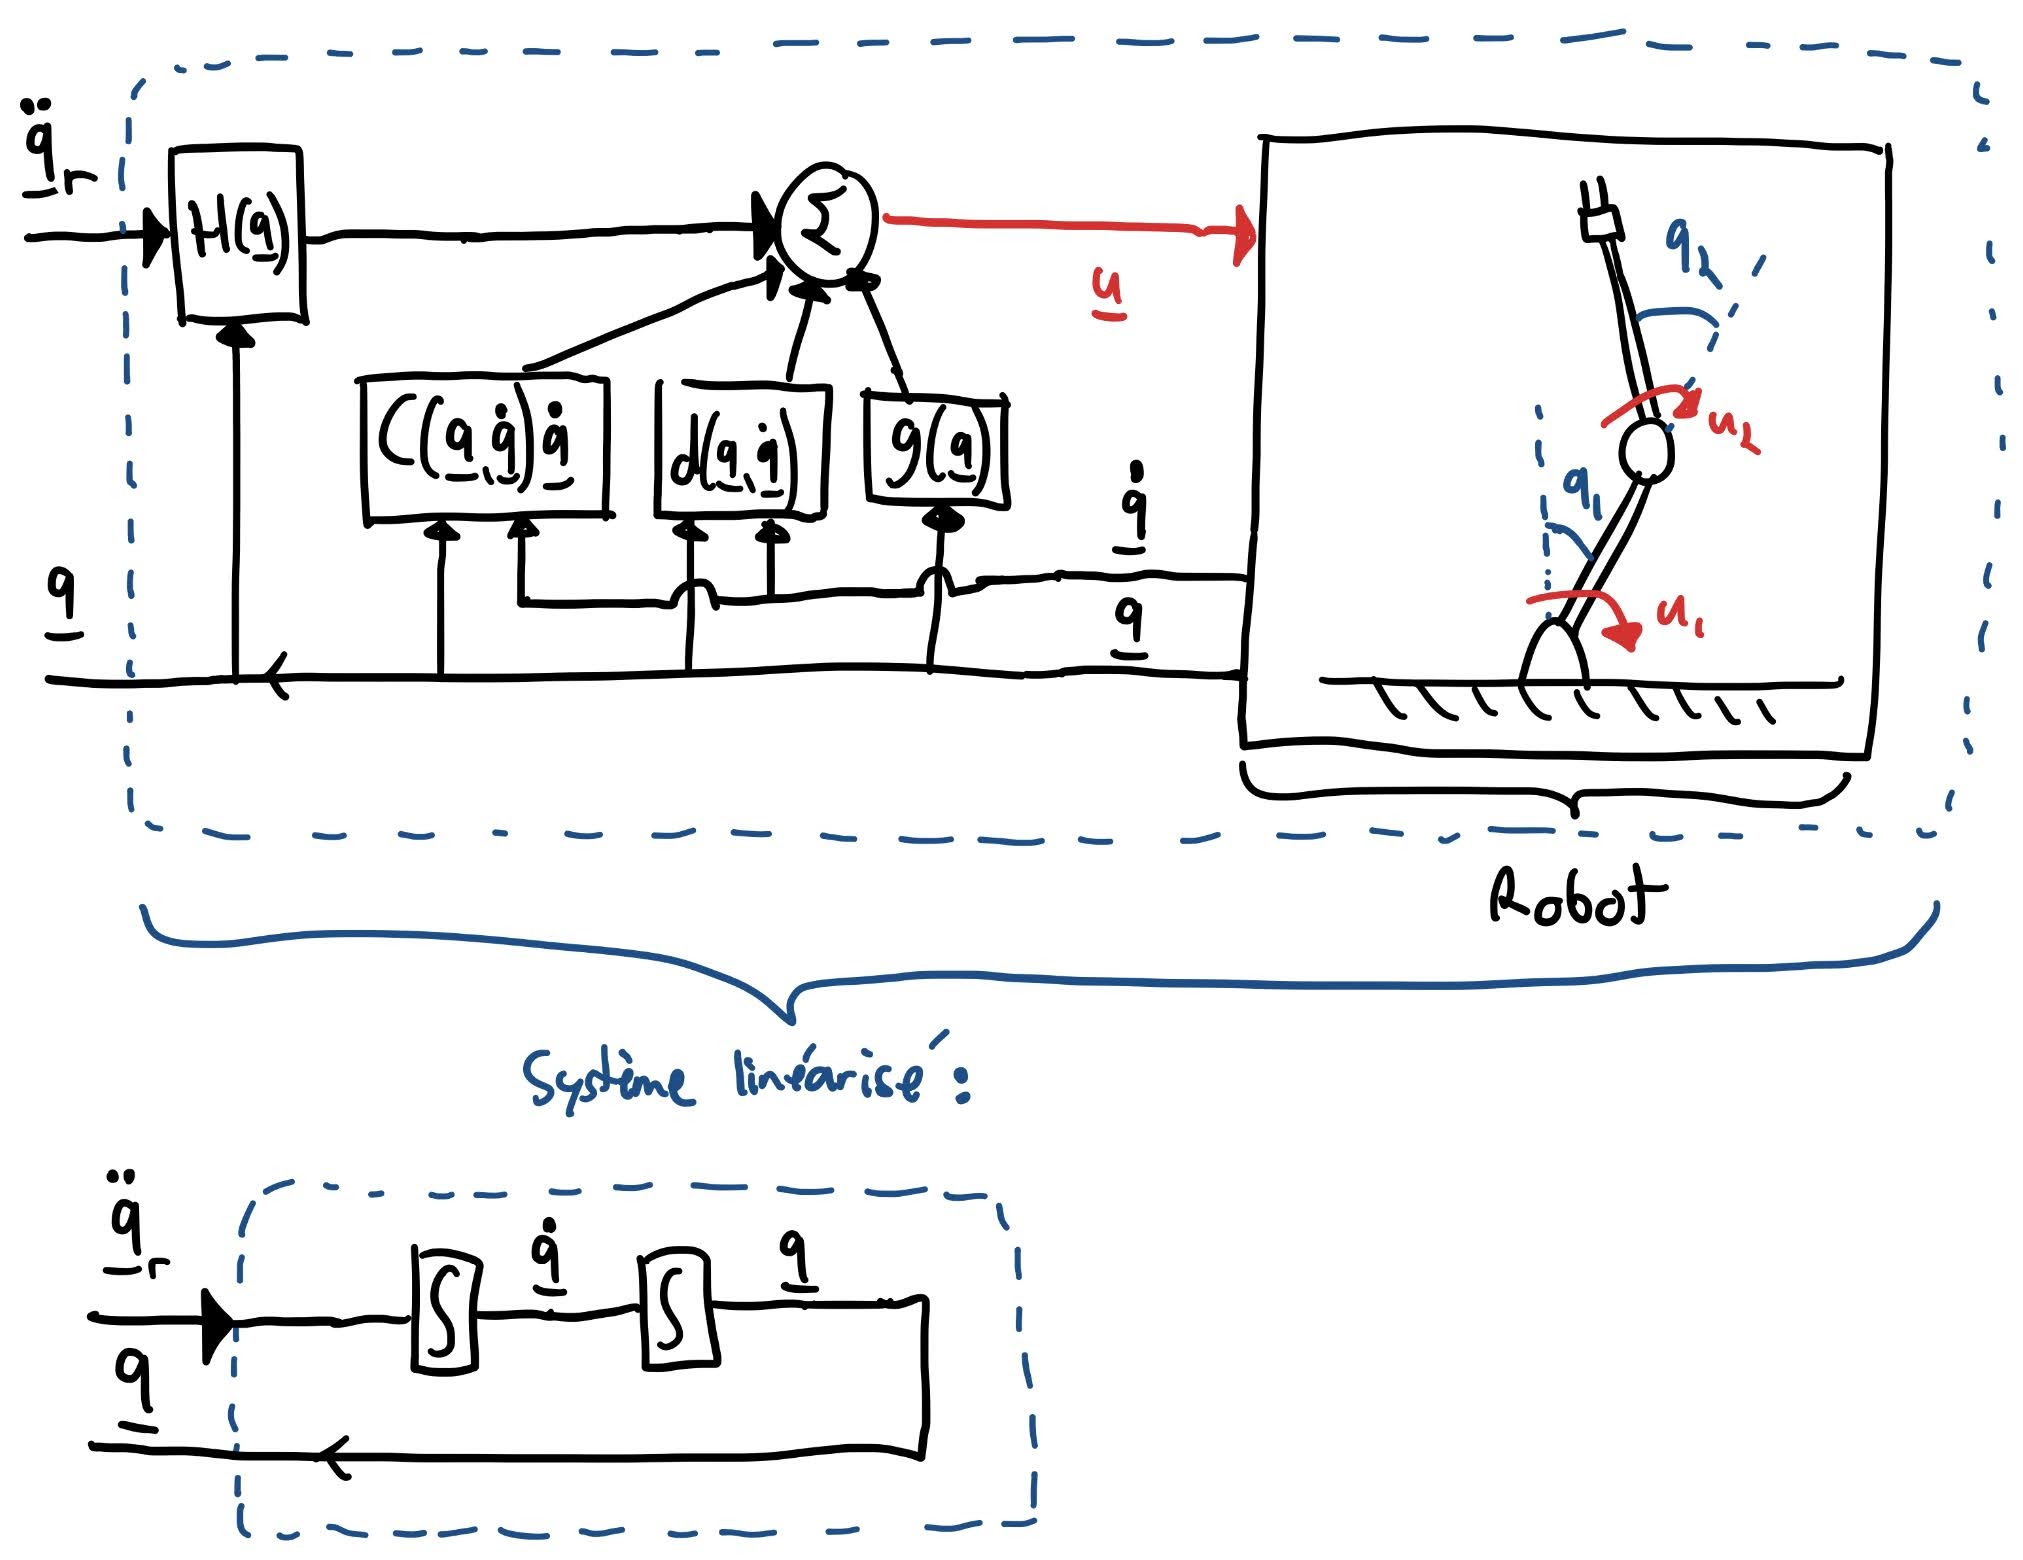
\includegraphics[width=0.75\textwidth]{fig/computedtorque.jpg}
	\caption{Couple calculé et boucle linéarisante}
	\label{fig:computedtorque}
\end{figure}
%%%%%%%%%%%%%%%%%%%%

\subsection{Suivi de trajectoire avec le couple calculé}

Lorsqu'on désire qu'un robot suivre une certaine trajectoire, il est possible de définir la référence d'accélération $\col{\ddot{q}}_r$ comme une fonction de la trajectoire cible pour obtenir que le robot va converger sur la trajectoire. Si une trajectoire cible est définie comme une fonction du temps pour les coordonnées $\col{q}$ et leur deux premières dérivées:
%%%%%%%%%%%%%%%%%%%%%%%
\begin{align}
\text{Trajectoire désirée: } \col{\ddot{q}}_d(t) \quad \col{\dot{q}}_d(t) \quad \col{q}_d(t)
\end{align}
%%%%%%%%%%%%%%%%%%%%%%%
alors si on définie la référence d'accélération par la loi de commande suivante:
%%%%%%%%%%%%%%%%%%%%%%%
\begin{align}
\col{\ddot{q}}_r = \col{\ddot{q}}_d + 2 \zeta w 
\underbrace{\left( \col{\dot{q}}_d - \col{\dot{q}}\right)}_{ \col{\dot{q}}_e}
+ w^2
\underbrace{\left( \col{q}_d - \col{q}\right)}_{ \col{q}_e}
\end{align}
%%%%%%%%%%%%%%%%%%%%%%%
puisqu'on obtient $\col{\ddot{q}} = \col{\ddot{q}}_r$ avec la méthode du couple calculé, en combinant cette définition pour $\col{\ddot{q}}_r$ on va obtenir:
%%%%%%%%%%%%%%%%%%%%%%%
\begin{align}
\underbrace{\left( \col{\ddot{q}}_d - \col{\ddot{q}} \right)}_{ \col{\ddot{q}}_e}
 + 2 \zeta w 
\underbrace{\left( \col{\dot{q}}_d - \col{\dot{q}}\right)}_{ \col{\dot{q}}_e}
+ w^2
\underbrace{\left( \col{q}_d - \col{q}\right)}_{ \col{q}_e} = 0
\end{align}
%%%%%%%%%%%%%%%%%%%%%%%
ce qui représente une équation de la dynamique pour l'erreur d'ordre 2 qui converge exponentiellement vers zéro, ce qui implique que la trajectoire du robot va converger sur la trajectoire désirée.

%%%%%%%%%%%%%%%%%%%%%%%%%
\begin{figure}[H]
	\centering
		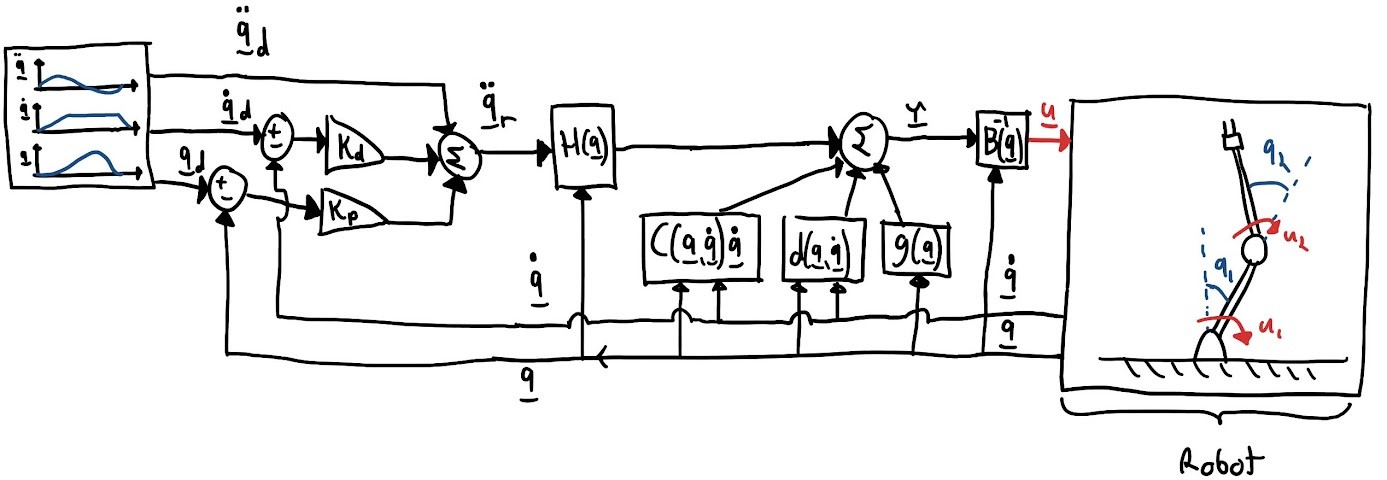
\includegraphics[width=0.99\textwidth]{fig/computedtorquetraj.jpg}
	\caption{Commande par couple calculé pour suivre une trajectoire}
	\label{fig:computedtorquetraj}
\end{figure}
%%%%%%%%%%%%%%%%%%%%

%%%%%%%%%%%%%%%%%%%%%%%%%
\begin{figure}[H]
	\centering
		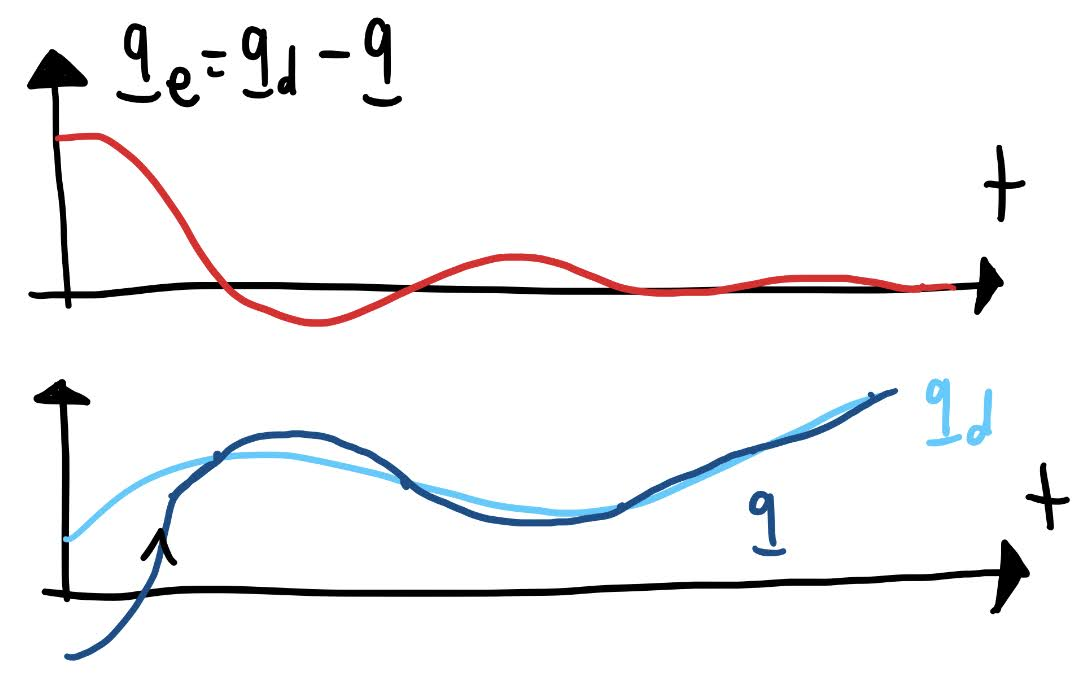
\includegraphics[width=0.50\textwidth]{fig/errordynamic.jpg}
	\caption{Dynamique de l'erreur et convergence sur la trajectoire}
	\label{fig:errordynamic}
\end{figure}
%%%%%%%%%%%%%%%%%%%%


\subsection{Suivi d'une trajectoire définie dans l'espace de la tâche}


\subsection{Limites de la méthode}


\subsection{Commande en impédance incluant les effets inertiels }

TODO voir notes manuscriptes alex 3 juillet 2022

\newpage
%%%%%%%%%%%%%%%%%%%%%%%%%%%%%%%%%%%%%%%%%%%%%%%
\section{Commande robuste}
%%%%%%%%%%%%%%%%%%%%%%%%%%%%%%%%%%%%%%%%%%%%%%%

\subsection{Méthode du mode glissant}

\video{Commande avec le mode glissant}{https://youtu.be/0Asg81SBjmk}


\newpage
%%%%%%%%%%%%%%%%%%%%%%%%%%%%%%%%%%%%%%%%%%%%%%%
\section{Commande adaptative}
%%%%%%%%%%%%%%%%%%%%%%%%%%%%%%%%%%%%%%%%%%%%%%%

\video{Exemple de loi de commande adaptative}{https://youtu.be/vmYjad6SOmU}


\section{Commande hybride en position et force}


\newpage
%%%%%%%%%%%%%%%%%%%%%%%%%%%%%%%%%%%%%%%%%%%%%%%
\section{Analyse de stabilité}
%%%%%%%%%%%%%%%%%%%%%%%%%%%%%%%%%%%%%%%%%%%%%%%

\video{Introduction à l'analyse de stabilité pour les systèmes non-linéaires}{https://youtu.be/q0Oqa5J3zEk}


\newpage
%%%%%%%%%%%%%%%%%%%%%%%%%%%%%%%%%%%%%%%%%%%%%%%
\section{Commande optimale}
%%%%%%%%%%%%%%%%%%%%%%%%%%%%%%%%%%%%%%%%%%%%%%%

\video{Exemple de loi de commande optimale pour un double intégrateur}{https://youtu.be/wKjEAXFvXlQ}

\video{Exemple de loi de commande optimale pour un pendule}{https://youtu.be/iUlkKdEK_dU}

\colab{Démo d'introduction aux méthodes de commande optimales}{https://colab.research.google.com/drive/1wXmlIqNGC2LrJkmyj56Y109b5ZDHVboq?usp=sharing}